\documentclass[10pt,twocolumn]{article}

\usepackage[a4paper,margin=17mm,columnsep=6mm]{geometry}
\usepackage[T1]{fontenc}
\usepackage{mathptmx}
\usepackage[scaled=0.9]{helvet}
\usepackage{courier}
\usepackage{microtype}
\usepackage{booktabs,tabularx,multirow}
\usepackage{xcolor}
\usepackage{tikz}
\usetikzlibrary{arrows.meta,positioning,fit,backgrounds,calc}
\usepackage{pgfplots}
\pgfplotsset{compat=1.17}
\usepackage{caption}
\captionsetup{font=small,labelfont=bf}
\usepackage[hidelinks]{hyperref}
\usepackage{url}
\usepackage{enumitem}
\setlist{nosep,leftmargin=*}

\definecolor{hblue}{HTML}{2A5C8A}
\definecolor{horange}{HTML}{C8742B}

\newcommand{\req}[1]{\textsf{#1}}

\title{\Large\bfseries Twenty Years On: Rebuilding a Robocode Robot with Agents\\[2pt]
\large A steel thread from college craft to the RoboRumble top 15, and what the human still does}

\author{Leigh Griffin\thanks{Corresponding author. %
% TODO(Leigh): affiliation and contact address.
Source, requirements, bench reports and data: \url{https://github.com/lgriffin/Hadur_Robot}.}}

\date{Draft, 8 October 2026}

\begin{document}
\maketitle

\begin{abstract}
\noindent Robocode was, for a generation of computing students, the first program that fought back:
a tank written in Java that had to sense, move, aim and survive against someone else's code. It
taught event-driven design, geometry, testing and, above all, measuring before believing. Twenty
years later we return to it with agentic software engineering. Over twelve days, a multi-agent
project of Claude Code sessions, steered by one developer, rebuilt the robot Hadur through 14
releases and over 100 merged pull requests, traced to about 210 EARS requirements and gated by a headless
bench. Hadur rose from 64th to 13th of about 1,216 robots in the 1v1 RoboRumble, and entered the
melee and team ladders (19th and 12th). We chart that history as a \emph{steel thread}: one
repeated loop of goal, staged plan, requirements, implementation, bench gate, release and live
reading. We report what accelerated, where the agents' own measurements were wrong, and which
decisions stayed with the human. Our claim is modest and, we think, useful: the skills Robocode
taught have not changed. What changed is where the developer spends them.
\end{abstract}

\section{Introduction}

Robocode \cite{robocode} has been used to teach programming and artificial intelligence since
IBM released it in 2001 \cite{hartness2004,okelly2006}. Its appeal is that the feedback is
immediate and unarguable: a robot either survives the round or it does not. Underneath the game,
a student meets the core of the craft. There is an event loop with a strict time budget per turn,
physics to model exactly, noisy sensors, an adversary that adapts, and a public ladder, the
RoboRumble \cite{roborumble}, that ranks every entry against every other over thousands of
battles. Many of us wrote our first serious Java there.

This paper is about returning to that robot twenty years later with a different way of working.
Hadur began as a robot that evolved by feel (Section~\ref{sec:background}). In
September and October 2026 it was rebuilt almost entirely by Claude Code agents working in a
multi-agent project: planning sessions wrote staged plans, implementation sessions wrote the
code, tests and bench reports, and one human set the goals, made the calls and acted in the
world on the project's behalf. The result climbed from 64th to 13th of about 1,216 robots in the
1v1 RoboRumble in ten days (Fig.~\ref{fig:aps}).

The rank is not the point, though it keeps us honest. The point is the thesis behind the project:
\emph{the skills that Robocode taught have not changed, and agentic development can still proceed,
accelerate and learn when those skills are applied deliberately}. Requirements still have to be
stated so they can be tested. Architecture still decides what can be tested at all. A claim still
needs a measurement, and a measurement still needs a control. What an agent changes is the cost of
the typing between those decisions, which falls close to zero, and so the decisions themselves
become the work.

We make three contributions.
\begin{enumerate}
\item A \textbf{steel thread} for agentic development of a measured system: one loop, repeated for
  every stage, from goal to live reading (Section~\ref{sec:thread}). It was used unchanged across
  six plans and about forty stages.
\item A \textbf{history with the data}: the architecture's evolution, the bench results and the live
  ladder, each traceable to a file in the public repository \cite{hadurrepo}
  (Sections~\ref{sec:arch} and~\ref{sec:history}).
\item \textbf{Insights on the human's role}, drawn from where the agents' plans and measurements
  were right, where they were wrong, and who noticed (Sections~\ref{sec:insights}
  and~\ref{sec:human}).
\end{enumerate}

\section{Background}\label{sec:background}

\paragraph{Robocode and the rumble.} A Robocode battle runs in discrete turns. Each turn a robot
receives events (a scan, a hit, a wall) and issues orders (turn, move, aim, fire, radar). Bullets
cost energy and refund three times their power on a hit; a robot that runs out of energy is
disabled. A robot cannot see bullets, only the opponent's energy, so it must infer when the
opponent fired from a drop in energy. The top robots \emph{wave surf}: they treat each inferred
shot as an expanding circle and move to where the opponent's gun is least likely to aim
\cite{robowiki}. The RoboRumble pairs every robot with every other and scores each pairing by
average percentage score (APS), the share of the pair's total score; a robot's rating is the mean
over about 1,215 pairings. There are separate ladders for 10-robot melee and 5-robot teams.

\paragraph{Hadur 1.x.} Hadur was a dual-mode duel and melee robot. Its later releases (1.17 to
1.20, ported to a Maven build in May 2026) used wave surfing, k-nearest-neighbour guess-factor
guns with 13 features, an anti-surfer gun and bullet shadows. It was strong but opaque. It was also
not hand-written in the old sense: 26 of its May commits carry a Claude co-author line. It was built
with one assistant in single sessions, by feel, and its own commit messages report progress as
rounds won against Shadow (``about 49\%''). It had
three weaknesses that shaped everything after: nothing measured it, so a gain could not be told
from noise; strategy was fused with the engine, so tactics could not be unit tested or replayed;
and its picture of the enemy was noisy, because it surfed waves that never existed.

\paragraph{The agentic setting.} The rebuild ran in a Claude Code project: a shared space where a
coordinator agent watches the project chat and starts a \emph{thread session} for each piece of
work. Each thread is a separate agent with its own repository checkout, and all share a project
memory and a file store. Over the twelve days, 33 threads ran. As a standing rule, a larger model
wrote the staged plans and a faster model implemented the stages. Every change reached the
repository as a pull request, and an automated reviewer commented on each one. The human, the
author, posted requests in the project chat, answered decision cards, and did the things only
a person could do (Section~\ref{sec:human}).

\paragraph{Two eras, one assistant.} Fig.~\ref{fig:activity} shows both eras. The assistant was Claude in
both. What changed in September was the way of working: a bench before any
change, requirements with IDs, an architecture that could be replayed, and a multi-agent project
that could run several stages at once. The rate of merged work rose about fivefold, from 1.6 to 8.7 pull requests a day, and, more
importantly, every merge after S0 came with a measurement.

\begin{figure}[t]
\centering
% Pull requests merged to master per day, from `git log --first-parent`. Both eras used
% Claude (26 commits in May carry a Claude co-author line); the second used the multi-agent
% project and the steel thread. Days with no merges are omitted.
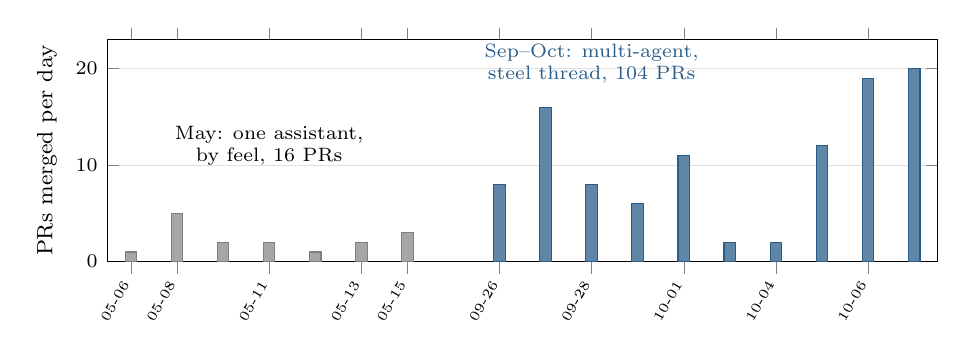
\begin{tikzpicture}
\begin{axis}[
  width=\columnwidth, height=4.4cm,
  ybar, bar width=4.2pt,
  symbolic x coords={05-06,05-08,05-09,05-11,05-12,05-13,05-15,gap,09-26,09-27,09-28,09-29,10-01,10-03,10-04,10-05,10-06,10-07},
  xtick={05-06,05-08,05-11,05-13,05-15,09-26,09-28,10-01,10-04,10-06},
  xticklabel style={rotate=60, anchor=east, font=\tiny},
  ylabel={PRs merged per day},
  ymin=0, ymax=23,
  ymajorgrids, grid style={black!12},
  tick label style={font=\scriptsize}, label style={font=\footnotesize},
  enlarge x limits=0.03,
  clip=false,
]
\addplot[fill=black!35, draw=black!50, bar shift=0pt] coordinates {
  (05-06,1) (05-08,5) (05-09,2) (05-11,2) (05-12,1) (05-13,2) (05-15,3) };
\addplot[fill=hblue!75, draw=hblue, bar shift=0pt] coordinates {
  (09-26,8) (09-27,16) (09-28,8) (09-29,6) (10-01,11) (10-03,2) (10-04,2) (10-05,12) (10-06,19) (10-07,20) };
\node[font=\scriptsize, align=center, anchor=south] at (axis cs:05-11,9) {May: one assistant,\\by feel, 16 PRs};
\node[font=\scriptsize, align=center, anchor=south, color=hblue] at (axis cs:09-28,17.5) {Sep--Oct: multi-agent,\\steel thread, 104 PRs};
\end{axis}
\end{tikzpicture}

\caption{Pull requests merged per day. May (grey): Hadur 1.17 to 2.0 with one assistant and no
bench. September to October (blue): the multi-agent project and the steel thread. Days without
merges are omitted.}
\label{fig:activity}
\end{figure}

\section{The steel thread}\label{sec:thread}

A steel thread is the thinnest end-to-end path through a system that exercises every layer, in the
spirit of the walking skeleton \cite{freeman2009}. Ours is a path through the \emph{process}, not
the code: one loop that every stage follows, from a goal to a reading of the live ladder
(Fig.~\ref{fig:thread}). It was set at the start and then not changed, which is what made the
pace safe.

\begin{figure}[t]
\centering
\resizebox{\columnwidth}{!}{% The steel thread: one loop per stage. Human-owned steps are shaded orange.
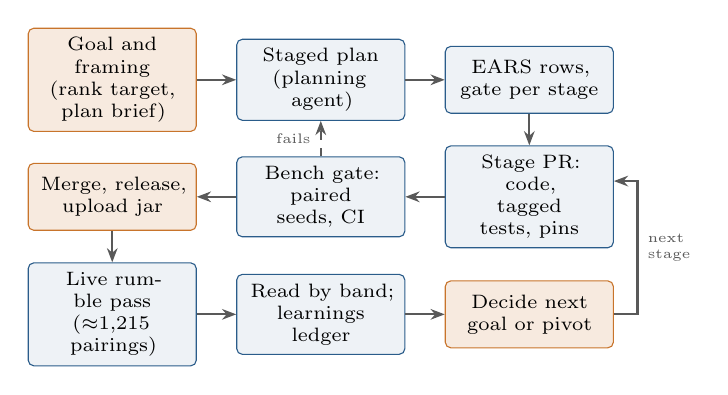
\begin{tikzpicture}[
  node distance=4mm and 5mm,
  box/.style={draw=hblue, fill=hblue!8, rounded corners=2pt, align=center,
    font=\scriptsize, minimum height=8.5mm, text width=19mm},
  hum/.style={box, draw=horange, fill=horange!15},
  arr/.style={-{Stealth[length=1.8mm]}, thick, black!65},
]
\node[hum] (goal) {Goal and framing\\(rank target, plan brief)};
\node[box, right=of goal] (plan) {Staged plan\\(planning agent)};
\node[box, right=of plan] (ears) {EARS rows,\\gate per stage};
\node[box, below=of ears] (impl) {Stage PR: code,\\tagged tests, pins};
\node[box, left=of impl] (gate) {Bench gate:\\paired seeds, CI};
\node[hum, left=of gate] (merge) {Merge, release,\\upload jar};
\node[box, below=of merge] (live) {Live rumble pass\\($\approx$1,215 pairings)};
\node[box, right=of live] (read) {Read by band;\\learnings ledger};
\node[hum, right=of read] (decide) {Decide next\\goal or pivot};
\draw[arr] (goal) -- (plan);
\draw[arr] (plan) -- (ears);
\draw[arr] (ears) -- (impl);
\draw[arr] (impl) -- (gate);
\draw[arr] (gate) -- (merge);
\draw[arr] (merge) -- (live);
\draw[arr] (live) -- (read);
\draw[arr] (read) -- (decide);
\draw[arr] (decide.east) -- ++(3mm,0) |- ([yshift=2mm]impl.east) node[pos=0.25, right, font=\tiny, align=left] {next\\stage};
\draw[arr, dashed] (gate.north) -- node[left, font=\tiny] {fails} (plan.south);
\end{tikzpicture}
}
\caption{The steel thread. Every stage of every plan ran this loop. Orange steps are the human's;
blue steps were done by agents. A failed gate returns to the plan, not to the code.}
\label{fig:thread}
\end{figure}

\paragraph{Goal and plan.} Each plan began with a goal stated by the human: a rank (top 30, then
top 15, then top 10), a capability (a robot that remembers each opponent), or a design brief (one
identity across three ladders). A planning agent turned it into stages, each small enough for one
pull request and each with a \emph{gate}: a bench result that must hold before the stage merges.
Plans were written as shareable documents and copied into the repository when they started, so
that the plan and its record could later be compared.

\paragraph{Requirements.} Every behaviour is an EARS requirement \cite{mavin2009}: ``\emph{When} an
enemy energy drop is not explained by the ledger, \emph{the robot shall} create a wave of the
remaining power.'' EARS suits agents well. Its fixed shapes (ubiquitous, event-driven,
state-driven, unwanted behaviour) leave little room to be vague, and each row carries an ID
(\req{WAVE-1}, \req{RAM-3}) that the tests must name. The repository holds about 210 distinct IDs.

\paragraph{Implementation.} An implementation agent builds one stage per pull request. The
rule is that each requirement due by the current stage has a Cucumber scenario tagged with its ID.
Pure logic gets unit tests and jqwik property tests \cite{claessen2000}. A change in recorded play
must be explained, and the replay fixtures re-recorded by name.

\paragraph{Gate.} The bench runs the real Robocode engine headless, one battle per process, with
fixed seeds. A gate compares a candidate jar with a baseline jar on the same seeds and opponents
(paired), and reports a mean difference with a 95\% interval. A stage merges when its gate holds;
when it does not, the stage goes back to the plan, or merges with the miss written down
(Section~\ref{sec:insights}).

\paragraph{Release and live reading.} Releases are cut by a workflow, and the human enters the jar
on the rumble's participants page. A full live pass takes an afternoon. The saved pages are parsed
into the repository's data archive, read by opponent rank band, and every finding goes into a
learnings ledger with its evidence and a status (confirmed, open or refuted). Findings that need
a decision about the bench itself get a 5 Whys record in a kaizen register \cite{sobek2008}.

\paragraph{Keeping it honest.} Table~\ref{tab:honesty} lists the layers that stop the documents,
tests and code from drifting apart. None is new. Together they let an agent change a codebase of about 37,000 lines of Java many times a day while a human reads only the summaries.

\begin{table}[t]
\centering
\caption{The layers that keep strategy, requirements and code aligned. Each fails the build or
the merge when it is violated.}
\label{tab:honesty}
\small
\begin{tabularx}{\columnwidth}{@{}lX@{}}
\toprule
Layer & What it guards \\
\midrule
EARS rows & What the robot must do, stage by stage \\
Traceability test & Every requirement due by the current stage names a test; unknown tags fail \\
ArchUnit & No Robocode, randomness, clock, threads or I/O in the core \\
Property tests & Physics equals the engine's; the ledger recovers exact shot power \\
Cucumber & One scenario per requirement, tagged with its ID \\
Replay & 13 recorded battles reproduce the live robot's orders bit for bit \\
Source pins & Hashes of each strand's packages; a change must re-pin by name \\
Bench gate & Paired score difference against the previous release \\
Live ladder & The rumble's full pass, read by band \\
\bottomrule
\end{tabularx}
\end{table}

\section{Architecture}\label{sec:arch}

\paragraph{Hexagonal core.} The first stage after the baseline (S1) moved every line of strategy
into a core with no Robocode imports, without changing how the robot played. A thin adapter turns
engine events into plain records (\texttt{BotInput}); the core returns \texttt{BotOrders}; and
telemetry and the profile store leave through ports \cite{cockburn2005}. A guard wraps the core:
if it throws, the robot still receives safe orders and the fault is counted. The port was proved
faithful by replay. Recorded battles against the reference opponents replay through a fresh core
to the live robot's exact orders. Comparing same-seed battles turn by turn against 1.20 exposed
two slips in the port, an angle read in degrees rather than radians and a gun-heat read one shot
late, and both were fixed before anything else changed.

This split is what made agentic work safe. An agent can change the gun and know within minutes
whether recorded play moved, and whether it moved only where the stage said it would.

\paragraph{One identity, three strands.} By robot 3.5.1 the core had grown a problem that was about
ownership, not speed. \texttt{HadurCore} was 2,100 lines and about 90 fields, two thirds of them
duel state. Melee was a delegate, a team was impossible, because in a team battle a teammate reads
as an opponent, and every new role would add branches to every event handler. The human's brief
for the next plan was short:

\begin{quote}\small
``I want an architecture evolution for Hadur using my hexagonal approach. There are three goals:
1v1, melee and team. All are attainable. [\dots] It knows its role, it adapts instantly, and it
does not have to guess or switch.''
\end{quote}

The planning agent turned that into six stages (A0 to A5) and five tests taken from the brief
(Fig.~\ref{fig:arch}). The battle's facts fix a \emph{charter} at tick 0. A pure function, the
role resolver, picks the role from the charter and three counts, and within a round it may only
step down a ladder: Team, then Melee, then Duel. Every role the charter allows is built and warmed
up before the first tick. The melee tracker became the kernel's single \emph{World}, which
teammates can also feed. Every package, output channel, memory file and requirement has exactly one
owner, enforced by per-strand source hashes. The duel's nine packages did not change in code from
A1 to A4, and no replay fixture was re-recorded. The evolution shipped as 3.7 with a second jar,
a five-robot team.

\begin{figure*}[t]
\centering
\resizebox{0.92\textwidth}{!}{% Hadur 3.9: an outer hexagon (adapter, guard, ports) around an identity kernel with
% three strands. Source: docs/architecture.md, docs/architecture-evolution.md.
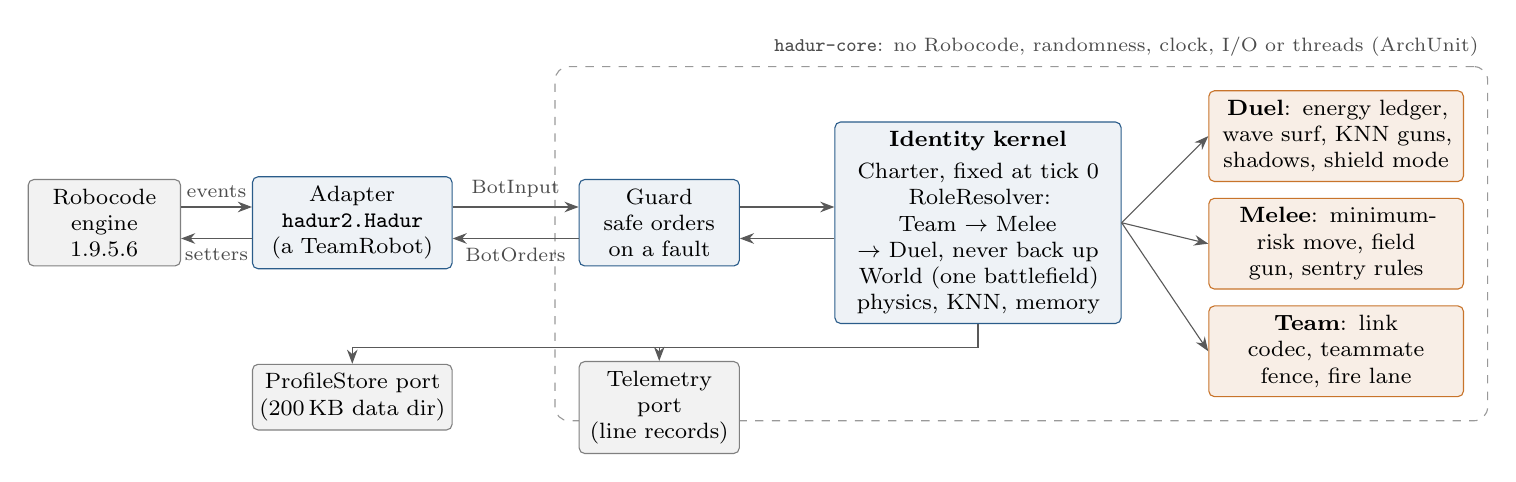
\begin{tikzpicture}[
  font=\footnotesize,
  box/.style={draw=hblue, fill=hblue!8, rounded corners=2pt, align=center, minimum height=9mm},
  ext/.style={draw=black!50, fill=black!5, rounded corners=2pt, align=center, minimum height=9mm},
  strand/.style={draw=horange, fill=horange!12, rounded corners=2pt, align=center,
    minimum height=9mm, text width=30mm},
  arr/.style={-{Stealth[length=1.8mm]}, black!65},
  lbl/.style={font=\scriptsize, black!70},
]
\node[ext, text width=17mm] (eng) {Robocode\\engine 1.9.5.6};
\node[box, right=9mm of eng, text width=23mm] (adp) {Adapter\\\texttt{hadur2.Hadur}\\(a TeamRobot)};
\node[box, right=16mm of adp, text width=18mm] (guard) {Guard\\safe orders\\on a fault};
\node[box, right=12mm of guard, text width=34mm, minimum height=24mm] (kern)
  {\textbf{Identity kernel}\\[2pt] Charter, fixed at tick 0\\ RoleResolver: Team $\rightarrow$ Melee\\$\rightarrow$ Duel, never back up\\ World (one battlefield)\\ physics, KNN, memory};
\node[strand, right=11mm of kern, yshift=11mm] (duel) {\textbf{Duel}: energy ledger, wave surf, KNN guns, shadows, shield mode};
\node[strand, below=2mm of duel] (melee) {\textbf{Melee}: minimum-risk move, field gun, sentry rules};
\node[strand, below=2mm of melee] (team) {\textbf{Team}: link codec, teammate fence, fire lane};
\draw[arr] ([yshift=2mm]eng.east) -- node[lbl, above]{events} ([yshift=2mm]adp.west);
\draw[arr] ([yshift=-2mm]adp.west) -- node[lbl, below]{setters} ([yshift=-2mm]eng.east);
\draw[arr] ([yshift=2mm]adp.east) -- node[lbl, above]{BotInput} ([yshift=2mm]guard.west);
\draw[arr] ([yshift=-2mm]guard.west) -- node[lbl, below]{BotOrders} ([yshift=-2mm]adp.east);
\draw[arr] ([yshift=2mm]guard.east) -- ([yshift=2mm]kern.west);
\draw[arr] ([yshift=-2mm]kern.west) -- ([yshift=-2mm]guard.east);
\foreach \s in {duel,melee,team} \draw[arr] (kern.east) -- (\s.west);
\node[ext, below=12mm of adp, text width=23mm, minimum height=7mm] (store) {ProfileStore port\\(200\,KB data dir)};
\node[ext, below=12mm of guard, text width=18mm, minimum height=7mm] (tel) {Telemetry port\\(line records)};
\coordinate (bus) at ($(kern.south)+(0,-3mm)$);
\draw[black!65] (kern.south) -- (bus) -- (bus -| store.north);
\draw[arr] (bus -| tel.north) -- (tel.north);
\draw[arr] (bus -| store.north) -- (store.north);
\begin{scope}[on background layer]
\node[draw=black!40, dashed, rounded corners=5pt, fit=(guard)(kern)(duel)(team), inner sep=3mm,
  label={[lbl, anchor=south east]north east:\texttt{hadur-core}: no Robocode, randomness, clock, I/O or threads (ArchUnit)}] {};
\end{scope}
\end{tikzpicture}
}
\caption{Hadur 3.9. The outer hexagon (adapter, guard, ports) dates from S1; the identity kernel
and its three strands from A1 to A5. The dashed boundary is enforced by ArchUnit on every build.}
\label{fig:arch}
\end{figure*}

\paragraph{Memory within a sandbox.} Robocode gives each robot 200\,KB of disk, forbids renaming
files, and charges for every byte written but refunds nothing on delete. Hadur keeps one profile
per opponent lineage, written with a CRC and a copy-then-delete protocol, and tests kill a save at
every byte of the file. The bench found that the delete protocol leaked quota (fixed by emptying a
file before deleting it, which the engine does refund). Live play later found something the bench
could not, which we return to in Section~\ref{sec:insights}.

\section{History}\label{sec:history}

Table~\ref{tab:plans} summarises the six plans and Fig.~\ref{fig:timeline} places them in time.
Each followed the loop of Fig.~\ref{fig:thread}.

\begin{figure*}[t]
\centering
\resizebox{\textwidth}{!}{% Plans and releases over the twelve days, 26 Sep to 7 Oct 2026 (day 0 = 26 Sep).
% Sources: docs/strategy-evolution.md, README.md rank history, project memory.
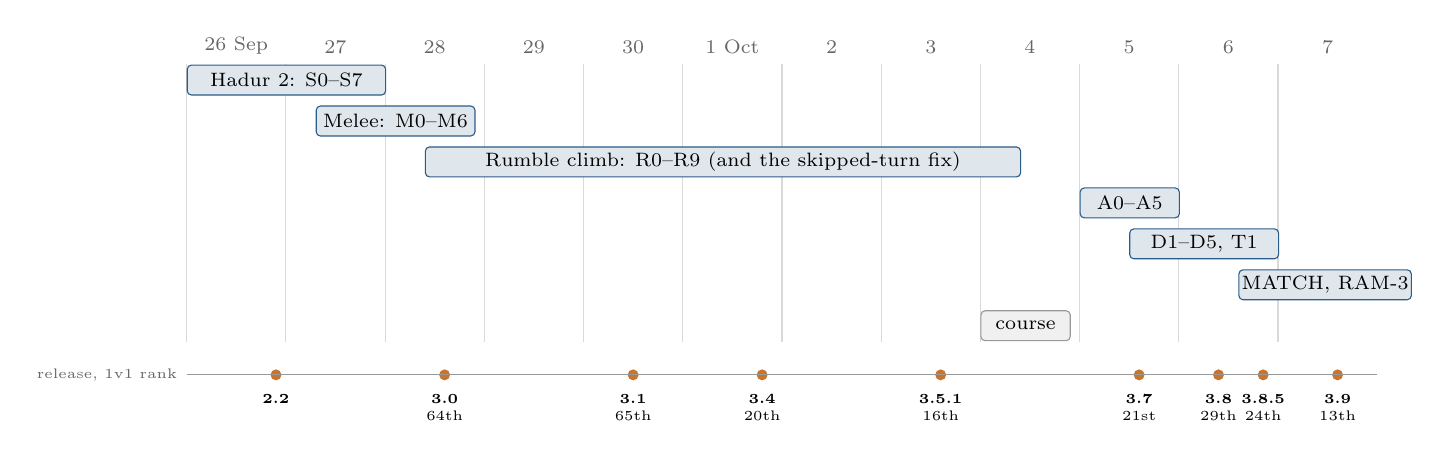
\begin{tikzpicture}[x=12.6mm, y=5.2mm, font=\scriptsize,
  plan/.style={draw=hblue, fill=hblue!15, rounded corners=1.5pt, minimum height=3.8mm, inner sep=1pt},
  rel/.style={circle, fill=horange, inner sep=1.4pt},
]
\foreach \d/\l in {0/26 Sep,1/27,2/28,3/29,4/30,5/1 Oct,6/2,7/3,8/4,9/5,10/6,11/7} {
  \draw[black!15] (\d,0.4) -- (\d,-6.4);
  \node[anchor=south, black!60] at (\d+0.5,0.4) {\l};
}
\node[plan, minimum width=2*12.6mm, anchor=west] at (0,0) {Hadur 2: S0--S7};
\node[plan, minimum width=1.6*12.6mm, anchor=west] at (1.3,-1) {Melee: M0--M6};
\node[plan, minimum width=6*12.6mm, anchor=west] at (2.4,-2) {Rumble climb: R0--R9 (and the skipped-turn fix)};
\node[plan, minimum width=1*12.6mm, anchor=west] at (9,-3) {A0--A5};
\node[plan, minimum width=1.5*12.6mm, anchor=west] at (9.5,-4) {D1--D5, T1};
\node[plan, minimum width=1.4*12.6mm, anchor=west] at (10.6,-5) {MATCH, RAM-3};
\node[plan, minimum width=0.9*12.6mm, anchor=west, draw=black!40, fill=black!6] at (8,-6) {course};
\foreach \x/\v/\r [count=\i] in {0.9/2.2/,2.6/3.0/64th,4.5/3.1/65th,5.8/3.4/20th,7.6/3.5.1/16th,9.6/3.7/21st,10.4/3.8/29th,10.85/3.8.5/24th,11.6/3.9/13th} {
  \node[rel] at (\x,-7.2) {};
  \node[anchor=north, align=center, font=\tiny] at (\x,-7.45) {\textbf{\v}\\\r};
}
\draw[black!40] (0,-7.2) -- (12,-7.2);
\node[anchor=east, font=\tiny, black!60] at (0,-7.2) {release, 1v1 rank};
\end{tikzpicture}
}
\caption{The twelve days. Bars are plans (grey: the companion course); dots are releases with the
1v1 rank of their first full pass. 2.2 was entered before the ladder was being read.}
\label{fig:timeline}
\end{figure*}

\begin{table*}[t]
\centering
\caption{The plans, in order. Dates are 2026. PR numbers are those of the public repository.}
\label{tab:plans}
\small
\begin{tabularx}{\textwidth}{@{}l l l X l@{}}
\toprule
Plan & Stages & Dates & What it delivered & Release \\
\midrule
Hadur 2 & S0--S7 & 26--27 Sep & Headless bench, hexagonal core, energy ledger, opponent memory, recognise-and-adapt, press-when-ahead, bullet shadows, tick budget (PRs \#18--\#32) & 2.1, 2.2 \\
Melee extension & M0--M6 & 27--28 Sep & Pinned duel, posture gate, melee radar and shot reading, minimum-risk movement with virtual bullets, learning field gun, melee memory & 3.0 \\
Rumble climb & R0--R9 & 28 Sep--3 Oct & Paired bench and stratified APS estimate, client reliability, full power vs weak bots, one-JVM session bench, skipped-turn fix, rammer escape (PRs to \#82) & 3.1--3.5.1 \\
Architecture evolution & A0--A5 & 5 Oct & Charter, role resolver, World, team ports and link, team baseline (PRs \#87--\#96) & 3.6, 3.7 \\
DrussGT route, Team & D1--D5, T1 & 5--6 Oct & Power by the lead, light-bullet gun, shadow-weighted aim, shield list; teammates that stop colliding (PRs \#98--\#105) & 3.8 \\
Leak repair & MATCH, RAM-3 & 6--7 Oct & Route scoped to duels not already won; rammer escape chosen per opponent (PRs \#116, \#130) & 3.8.5, 3.9 \\
\bottomrule
\end{tabularx}
\end{table*}

\paragraph{Measure first (S0 to S6).} The first stage changed nothing in the robot. It built the
bench and measured 1.20: against Shadow 3.83c, the reference duelist, Hadur won about half its
rounds but took only 40.8\% of the score. Score share, not rounds won, became the headline metric.
The stages that followed made the robot more correct before they made it stronger
(Fig.~\ref{fig:shadow}). S2 replaced ``any energy drop is a shot'' with an energy ledger that
accounts for every other cause of a drop. Scored against the engine's real bullets, it found
99.4\% of the shots a scan could reveal with no false waves, and explained away 1,820 drops that
1.20 had surfed as phantom shots. S3 and S4 gave the robot a crash-safe memory and let it adapt
to a remembered opponent, with tiers named only when an Agresti--Coull margin \cite{agresti1998}
was tight enough. None of these moved the score outside the noise, and the documents said so at
each stage. S6 did. Bullet shadows, the firing angles that our own bullets block, raised the
share to 57.4\%. It took three rounds of fixing the geometry against the engine's truth logs
(35\%, then 83\%, then 100\% of destroyed enemy bullets inside a computed shadow) before the
feature was trusted.

\begin{figure}[t]
\centering
% Score share against Shadow 3.83c by stage, cold bench, 35 rounds x 5 seeds,
% mean and 95% interval. Source: docs/strategy-evolution.md "Results by stage".
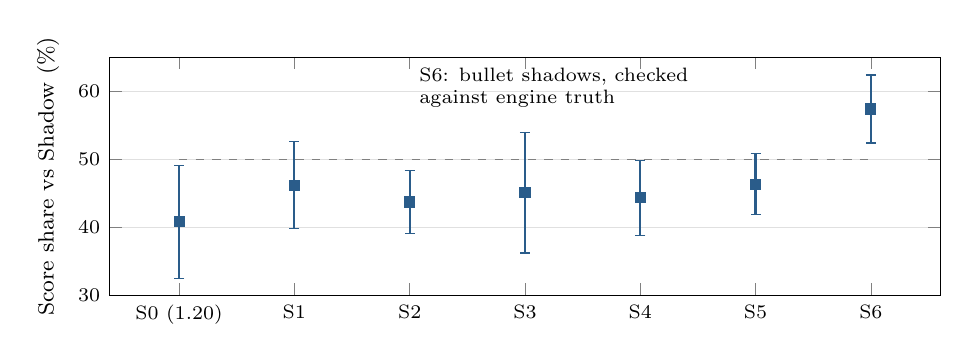
\begin{tikzpicture}
\begin{axis}[
  width=\columnwidth, height=4.6cm,
  symbolic x coords={S0,S1,S2,S3,S4,S5,S6},
  xtick=data,
  xticklabels={S0 (1.20), S1, S2, S3, S4, S5, S6},
  ylabel={Score share vs Shadow (\%)},
  ymin=30, ymax=65,
  ymajorgrids, grid style={black!12},
  tick label style={font=\scriptsize}, label style={font=\footnotesize},
]
\addplot[only marks, mark=square*, mark size=1.8pt, color=hblue,
  error bars/.cd, y dir=both, y explicit, error bar style={thick}] coordinates {
  (S0,40.8) +- (0,8.3) (S1,46.2) +- (0,6.4) (S2,43.7) +- (0,4.6) (S3,45.1) +- (0,8.9)
  (S4,44.3) +- (0,5.5) (S5,46.3) +- (0,4.5) (S6,57.4) +- (0,5.0)
};
\addplot[dashed, color=black!50] coordinates {(S0,50) (S6,50)};
\node[font=\scriptsize, anchor=west, align=left] at (axis cs:S2,60.5) {S6: bullet shadows, checked\\against engine truth};
\end{axis}
\end{tikzpicture}

\caption{Score share against Shadow 3.83c by stage (cold bench, 35 rounds $\times$ 5 seeds, 95\%
interval). Five stages of correctness work held the score level; S6 moved it.}
\label{fig:shadow}
\end{figure}

\paragraph{The live ladder disagrees (3.0 to 3.4).} 3.0 entered the rumble at 85.5 APS over its first 268
pairings and fell to 77.2 over the next 239; 3.1 slid the same way. The bench, at every CPU setting tried, could
not reproduce it. The learnings ledger recorded the gap as open and named the difference: the bench
forked a fresh JVM per battle and met at most 60 opponents, whereas a rumble client runs hundreds of
battles in one process with a data directory that grows by one profile per opponent. A
session bench built to match (R7) traced the slide to the round-end profile save, which scanned that
growing directory and caused skipped turns. 3.4 fixed it and held 85.9 APS, 20th.

\begin{figure}[t]
\centering
% 1v1 RoboRumble APS and rank by release. Source: README.md "Rank history",
% docs/bench/live-3.9.md (10th place on 2026-10-07 20:28 UTC).
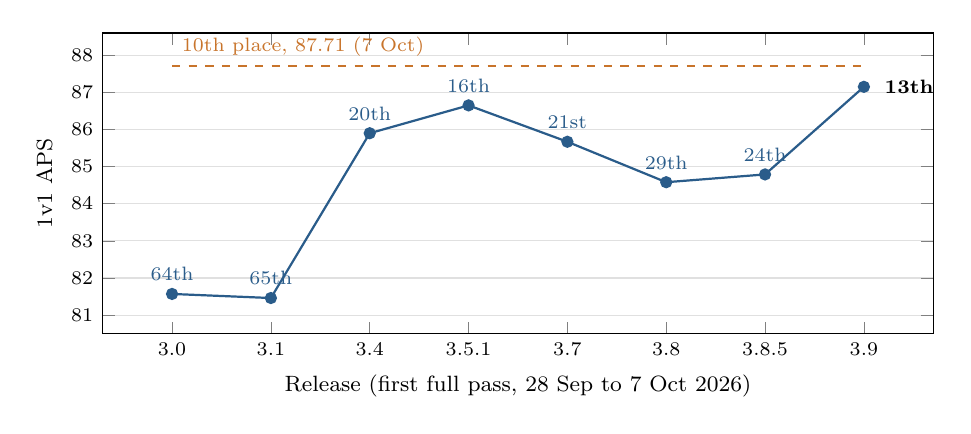
\begin{tikzpicture}
\begin{axis}[
  width=\columnwidth, height=5.4cm,
  symbolic x coords={3.0,3.1,3.4,3.5.1,3.7,3.8,3.8.5,3.9},
  xtick=data,
  xlabel={Release (first full pass, 28 Sep to 7 Oct 2026)},
  ylabel={1v1 APS},
  ymin=80.5, ymax=88.6,
  ytick={81,82,83,84,85,86,87,88},
  ymajorgrids, grid style={black!12},
  tick label style={font=\scriptsize}, label style={font=\footnotesize},
  nodes near coords={\scriptsize\pgfplotspointmeta},
  point meta=explicit symbolic,
  every node near coord/.append style={anchor=south, yshift=1pt},
  clip=false,
]
\addplot[thick, mark=*, mark size=1.8pt, color=hblue] coordinates {
  (3.0,81.57)[64th] (3.1,81.46)[65th] (3.4,85.90)[20th] (3.5.1,86.65)[16th]
  (3.7,85.67)[21st] (3.8,84.58)[29th] (3.8.5,84.79)[24th] (3.9,87.15)[]
};
\addplot[dashed, color=horange, thick] coordinates {(3.0,87.71) (3.9,87.71)};
\node[anchor=south west, font=\scriptsize, color=horange] at (axis cs:3.0,87.71) {10th place, 87.71 (7 Oct)};
\node[anchor=west, font=\scriptsize, xshift=4pt] at (axis cs:3.9,87.15) {\textbf{13th}};
\end{axis}
\end{tikzpicture}

\caption{1v1 RoboRumble APS and rank for each release's first full pass. The dip at 3.8 is the
DrussGT route's cost against the weak field; 3.9 recovers it.}
\label{fig:aps}
\end{figure}

\paragraph{A route to the top, and a leak (3.7 to 3.9).} With the architecture in place, the next
plan aimed at DrussGT, a long-time leader. The bench showed both robots' guns hitting below
break-even against each other, so the robot firing lighter bullets keeps its lead; D1 taught the
duel that, and the gate rose 12 points against DrussGT. 3.8 shipped five such stages. Live, it
gained 5.2 points per pairing against the top 10, where it was aimed, and fell to 29th. Against
every opponent ranked 21st and below it lost 1.55 points per pairing, mostly through lost rounds,
and with about 1,200 such pairings that outweighed the gain at the top. 3.8.5 scoped the route to
duels the robot was not already winning on the guns and recovered a fifth of the loss. A bisect of
releases on the opponents that had beaten 3.4 then put the remaining loss in 3.5's rammer escape,
not in the new route. 3.9 tries the escape for two rounds and then keeps, per opponent, whichever
of escape or fight paid. It reached 87.15 APS, Hadur's best, 13th, and 0.56 below 10th
(Fig.~\ref{fig:bands}).

\begin{figure}[t]
\centering
% 3.9 minus 3.8.5 per live pairing, by opponent rank band, 95% interval.
% Source: docs/bench/live-3.9.md. The paired bench gate on the 32-bot leak set read
% -0.02 (level); live on the same bots read +2.14 +- 1.04.
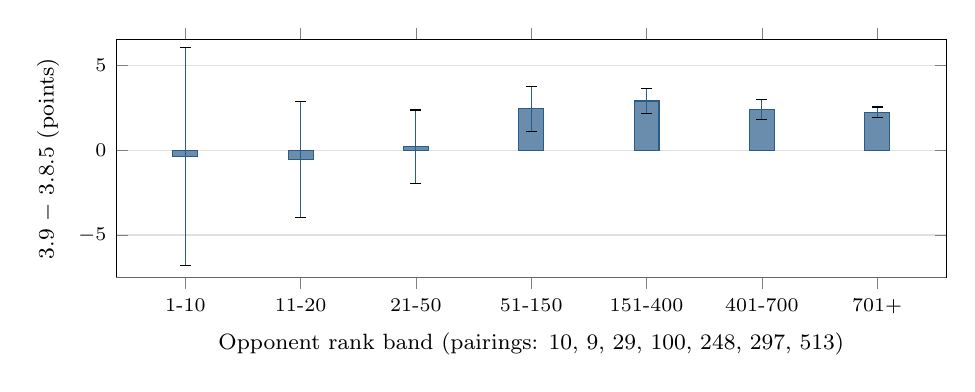
\begin{tikzpicture}
\begin{axis}[
  width=\columnwidth, height=4.6cm,
  symbolic x coords={1-10,11-20,21-50,51-150,151-400,401-700,701+},
  xtick=data,
  xlabel={Opponent rank band (pairings: 10, 9, 29, 100, 248, 297, 513)},
  ylabel={3.9 $-$ 3.8.5 (points)},
  ymin=-7.5, ymax=6.5,
  ymajorgrids, grid style={black!12},
  tick label style={font=\scriptsize}, label style={font=\footnotesize},
  ybar, bar width=9pt,
]
\addplot[fill=hblue!70, draw=hblue,
  error bars/.cd, y dir=both, y explicit] coordinates {
  (1-10,-0.37) +- (0,6.42) (11-20,-0.56) +- (0,3.43) (21-50,0.19) +- (0,2.17)
  (51-150,2.43) +- (0,1.31) (151-400,2.89) +- (0,0.73) (401-700,2.39) +- (0,0.59)
  (701+,2.24) +- (0,0.30)
};
\draw[black!60] (rel axis cs:0,0) -- (rel axis cs:1,0);
\end{axis}
\end{tikzpicture}

\caption{3.9 minus 3.8.5 per live pairing, by opponent rank band (95\% interval). The gain is even
across the field below rank 50 and comes from survival. The paired bench gate on 32 of these
opponents read level.}
\label{fig:bands}
\end{figure}

\paragraph{Melee and team.} The melee extension (M0 to M6) raised the reference-field APS from
37.9 to between 52.7 and 54.6, and firsts on a challenge field from 33 to 72 of 100. The team
baseline (A5) fielded five robots that shared sightings; its bench found about 440 teammate
collisions per round. T1 made teammates visible to each other's movement and added a fence that
brakes before a collision. On the gate, collisions fell from 101,322 to 65 and score share rose
from 28.8\% to 48.2\%. Live, the team went from 32nd of 46 to 12th, and the melee entry has held
between 16th and 19th of about 415 since 3.5.1.

\section{One turn of the thread: 3.9}\label{sec:example}

The last release shows the loop at full size, and where the human sits in it.

\begin{enumerate}[label=\arabic*.]
\item \textbf{Read.} 3.8.5's pass left Hadur 1.1 APS below 3.4, mostly in lost rounds against weak
  opponents. The agent listed the 40 bots that had beaten 3.4 in both passes.
\item \textbf{Bisect.} Whole releases (3.4, 3.5.1, 3.7, 3.8, 3.8.5) were benched in pairs on those
  bots. The only resolved step was 3.4 to 3.5.1: $-6.4$ points, with 14 of 39 opponents down after
  a Holm correction. A 5 Whys record noted that the set was chosen on 3.4's luck, so the size of the
  loss was uncertain even if its place was not.
\item \textbf{Cause.} 3.5's rammer escape (\req{RAM-2}) ran from robots that confirm as rammers but
  are really close-range fighters, and running, Hadur was hit two to seven times as often.
\item \textbf{Requirement.} \req{RAM-3}, state-driven: \emph{while} the enemy is a confirmed rammer,
  each round \emph{shall} play one arm from its start, the escape for two rounds, then whichever arm
  has the higher mean energy margin.
\item \textbf{Build and gate.} One class, \texttt{EscapeTrial}, a tagged scenario, a telemetry
  record per choice. The gate ran on the human's PC for the CPU: $+5.46$ on the live losers (ten up
  after Holm), level on the leak set and the top 20.
\item \textbf{Decide.} The agent offered ship or hold on a decision card, with its estimate:
  $+0.2$ to $+0.4$ APS. The human shipped.
\item \textbf{Live.} 87.15 APS, 13th: $+2.32$ APS, even across every band below rank 50
  (Fig.~\ref{fig:bands}). The estimate was low by a factor of six, and the bench on a wider set had
  read level. Both facts went into the ledger, with an open question: what in live play makes a
  rammer confirm on an ordinary bot?
\end{enumerate}

\section{Insights}\label{sec:insights}

\paragraph{1. The bench is necessary, and it is not the ladder.} Three times the bench and the
ladder disagreed, and each time the ladder was right: the 3.0 slide, the 3.8 leak, and 3.9's gain,
where the bench gate read $-0.02$ points on the 32-bot leak set and the live pass read $+2.14 \pm
1.04$ on the same bots. On the top of the ladder, by contrast, the bench predicts live play well
(correlation 0.96 over 18 of the top 19). The lesson is about selection, not tooling. Benches are
built from the opponents one is thinking about, and the rating is a flat mean over everyone. A
human who reads the whole ladder, band by band, finds what the bench was not built to see.

\begin{table}[t]
\centering
\caption{Three times the bench and the ladder disagreed. Each time the ladder was right, and the
fix was to the bench or to what it was asked.}
\label{tab:disagree}
\small
\begin{tabularx}{\columnwidth}{@{}l>{\raggedright\arraybackslash}X>{\raggedright\arraybackslash}X@{}}
\toprule
Release & Bench said & Ladder said \\
\midrule
3.0, 3.1 & 35/35 rounds on the worst live rows, at every CPU setting & Slide of 5 to 8 APS within hours; cause: a save scanning a growing data dir \\
3.8 & Top 10 $+7.2$; weak set level & 29th: top 10 $+5.2$, ranks 21+ $-1.55$ per pairing \\
3.9 & Leak set level ($-0.02$) & Same bots $+2.14 \pm 1.04$; field $+2.3$ APS \\
\bottomrule
\end{tabularx}
\end{table}

\paragraph{2. Ground truth turns tuning into engineering.} The most productive bench feature was
not a score. It was a per-turn log of the engine's true positions and bullets, against which every
inference could be checked. That turned ``the surfing feels better'' into ``13.6\% false waves
against Crazy, because the engine accelerates before its wall check'', and the shadow geometry from
35\% to 100\%. Agents are very good at closing a measured gap. They are much less good at
noticing that a gap exists when nothing measures it.

\paragraph{3. Review by another agent finds real bugs.} An automated reviewer read every pull
request. Its findings were often correct and often subtle. On one stage it showed that a new
power rule's margin was set so tight that a real 100-shot window could never satisfy it: the rule
passed its own tests but could never fire live. On another it caught a ram response whose power
override ignored whether the robot could afford the shot. Separating the author and the reviewer
of a change matters as much for agents as for people.

\paragraph{4. Agents report misses honestly when the process asks them to.} Not every stage met its
own measure. D3's light-bullet gun did not raise the hit rate it was built to raise
($+0.03 \pm 0.21$ points), and the record says so; it merged on the stack's combined gate. 3.9's
gate predicted $+0.2$ to $+0.4$ APS, and the ladder gave $+2.3$. Writing both numbers down, with the
rule that a refuted learning is marked and not deleted, is what lets the next plan start from the
truth.

\paragraph{5. Architecture is a prerequisite for speed.} Before S1, a change to the robot could
only be judged by watching battles. After S1 it could be replayed bit for bit; after A1 it could
be confined to one strand by source hashes. Each fixed point the architecture added let the agents
make larger changes with less risk. This is the oldest lesson in the field \cite{brooks1987}, and
it applies to agents with more force, because they make many more changes.

\paragraph{6. The agents' failure modes are specific, and checkable.} Across the record, the
agents' mistakes fell into a few kinds, each of which a process step caught:
\begin{itemize}
\item \emph{A rule that cannot fire.} Thresholds that pass unit tests but can never be met by live
  data (the power rule above). Caught by review against realistic windows.
\item \emph{Confident estimates.} Gate-based APS predictions were off by a factor of six in one
  direction (3.9) and by a sign in the other (3.8). Caught only by the live pass.
\item \emph{Selection on luck.} Opponent sets chosen because a release lost to them overstate the
  loss. Caught by a 5 Whys record and an unselected rerun.
\item \emph{Confounded hosts.} One stage's skipped turns rose twentyfold on a loaded machine
  (283 against 15). Caught because the report published per-tick timings, not only totals.
\item \emph{Stale artefacts.} A build that fails late can leave the previous jar in place, so a
  bench measures the wrong robot. Caught by checking the jar for the stage's classes before a run.
\end{itemize}
None of these is specific to agents. All are what a careful student learns to check, and all
become more frequent when changes are cheap.

\paragraph{7. The pace changes the bottleneck.} Over 100 pull requests merged in twelve days, with
61 commits on the busiest day. At that rate, the scarce resources are the live ladder (one full
pass per afternoon), compute for the bench (gates ran for hours, some on the author's own PC), and
the human's attention. The plans adapted: a release bundled several stages, and the live pass
became the gate that mattered most.

\section{The role of the human}\label{sec:human}

Table~\ref{tab:roles} lists who did what. We draw it from the project's own record (the plan
documents, decision cards and the project memory), not from memory of the work.

\begin{table}[t]
\centering
\caption{Who did what, over the twelve days.}
\label{tab:roles}
\small
\begin{tabularx}{\columnwidth}{@{}>{\raggedright\arraybackslash}p{0.41\columnwidth}X@{}}
\toprule
Human & Agents \\
\midrule
Set every goal (top 30, 15, 10) and brief & Wrote the staged plans and EARS rows \\
Chose pivots: park melee, keep it, add a team & Wrote the code, tests and fixtures \\
Picked between options on decision cards & Ran and wrote up every bench gate \\
Entered each release on the ladders; saved the live pages & Parsed the pages; read the pass by band \\
Ran long benches on a personal PC & Bisected releases; kept the ledger \\
Set conventions (what goes where, how to report) & Reviewed every PR; fixed findings \\
Pushed tags; edited the robot's wiki entries & Drafted release notes and docs \\
\bottomrule
\end{tabularx}
\end{table}

\paragraph{Intent.} Every plan started from a sentence the human wrote, and the best plans started
from the best sentences. The architecture brief above fits in four lines. It contains the whole
design test (know the role, adapt instantly, no guessing, no overlap, one identity), and the
planning agent's job was to make it concrete. When a goal was vague, such as ``climb the rumble'',
the first plan was too.

\paragraph{Judgement under uncertainty.} The agents produced options with evidence. The human chose.
Melee was parked on day one to focus on the duel, then kept when a port of the old melee brain
turned out to be cheap. 3.9 shipped on a decision card when its gate gained 5.5 points on the opponents that had beaten
3.4 live but read level on the wider sets. These are bets, and the agents framed them well, but the
judgement of which risks were worth taking with a public entry stayed with the person whose name
is on it.

\paragraph{Acting in the world.} Several steps could only be done by a person: entering a jar on
the participants page, saving the ladder's pages when a pass completed, editing the robot's country
flag on the community wiki, pushing tags, and running the longest benches on a machine with the
right CPU. These steps are mundane, and they are also the loop's connection to reality. Without
them, the agents would have optimised the bench indefinitely.

\paragraph{Noticing.} The 3.8 regression was raised by the human reading the ladder the afternoon it
landed. The agents had a passing release check, with a plus of 7.2 points on the top 10. A habit
from college Robocode, watching the whole rating and not only the opponents you care about, was
what found it.

\paragraph{What did not change.} Table~\ref{tab:skills} maps the skills a first Robocode project
teaches onto the moments in this history where they decided the outcome. Every decisive moment used
one of them: stating what the robot must do so that it can be
checked, separating the brain from the engine so that it can be tested, logging the truth and
comparing against it, distrusting a single battle, and reading the ladder. The agents brought
enormous throughput and real expertise in the domain's techniques. The human brought the same
craft that college taught \cite{mcbreen2001,hunt1999}, applied to specifying, measuring and
deciding rather than typing.

\begin{table}[t]
\centering
\caption{Skills a college Robocode project teaches, and where each decided the outcome here.}
\label{tab:skills}
\small
\begin{tabularx}{\columnwidth}{@{}>{\raggedright\arraybackslash}p{0.30\columnwidth}>{\raggedright\arraybackslash}X@{}}
\toprule
Skill & Where it decided the outcome \\
\midrule
Model the physics exactly & The ledger's 99.4\% shot recovery; the wall check that caused 13.6\% false waves \\
Separate brain from engine & S1's core made every later change replayable \\
Respect the turn budget & The 3.0 slide was skipped turns from a save \\
Log the truth, compare & Shadows from 35\% to 100\% against engine logs \\
Distrust one battle & Paired seeds, intervals, the 0.56 APS still to find \\
Read the whole ladder & The 3.8 leak, found by band, not by the gate \\
Say what it must do & EARS rows that a test must name \\
\bottomrule
\end{tabularx}
\end{table}

\section{Implications for teaching}

If Robocode is still an entry point, the question for a course is what students should now do
with it. Our record suggests an answer: keep the robot, change the deliverable. A student who
asks an assistant for a wave-surfing robot will get one, as Hadur 1.x shows. What the assistant
does not supply is the bench, the requirement IDs, the replay test, or the habit of reading the
whole ladder, and those are where every decisive moment in this history came from. A course can
make them the graded artefacts: a baseline measurement before any change, one EARS row and one
tagged test per behaviour, a paired gate with an interval, and a written reading of a live pass.
The companion course built alongside this work, 17 topics and 15 labs with a small teaching
robot, follows that structure; its evaluation is future work.

\section{Related work}

Robocode has a long record in teaching, as a vehicle for AI \cite{hartness2004} and for
problem-based learning in introductory programming \cite{okelly2006}. Code generation has reopened
the question of what novices must learn \cite{becker2023}, and controlled studies report large
speed-ups for individual tasks \cite{peng2023}. Agent benchmarks such as SWE-bench measure single
issue resolution \cite{jimenez2024,yang2024}, and multi-agent frameworks assign software roles to
cooperating models \cite{hong2024,qian2024}. Our setting differs in three ways: the system is long
lived and measured against an external, adversarial ladder; the agents work over many stages
against a shared requirements baseline; and the human remains in the loop as the owner of goals
and of contact with the world. We are not aware of an end-to-end account of that combination
with its data public.

\section{Threats to validity}

This is a single case with a single developer and one family of models, so the account is
illustrative, not general. The rumble is noisy: most pairings in a pass are one or two battles,
and other entries change while ours do. We report first full passes and intervals throughout, and
the band figures use the complete pass. Our attribution of roles relies on the project's own
records, which the agents wrote; we reduce that bias by citing decisions and data, not
characterisations. Finally, ``twelve days'' measures elapsed time, not effort: the agents ran for
many hours in parallel, and the benches for longer.

\section{Conclusion and next steps}

Twenty years on, Robocode is still a good teacher. Rebuilding Hadur with agents took it from 64th
to 13th of about 1,216 in twelve days, onto two more ladders, and through an architecture that
lets one identity play all three. The steel thread (goal, plan, requirements, implementation,
gate, release, live reading) did not change once in that time, and that stability is what let the
pace be safe. The work that mattered most was the oldest work in the craft. The agents made it
cheap to act on good decisions; they did not make the decisions less necessary.

The open target is the top 10, 0.56 APS away. The live data puts the remaining points in two groups
of weak opponents, close-range rammers that take a fifth of the score and simple guns that win
rounds they should not, and not at the top. A full version of this paper will report that climb,
an effort accounting, and the companion course built from the same history.

\bibliographystyle{plain}
\bibliography{refs}

\end{document}
